\begin{quoting}
Dans ce chapitre du livre, nous examinerons de plus près
les différents types de levain et leurs caractéristiques respectives.
\end{quoting}

\begin{table}[htp!]
    \begin{center}
        \begin{tabular}{@{}lclll@{}}
\toprule
                     &                         & &\multicolumn{2}{c}{\textbf{Activity}}\\
                                                                         \cmidrule(ll){4-5}
\textbf{Starter type} & \textbf{Hydration (\%)} & \textbf{Flour type}  & \textbf{Yeast} & \textbf{Bacterial} \\ \midrule
Regular              & 100                     & Strong wheat       & Balanced      & Balanced          \\ 
Liquid               & 500                     & Very strong wheat  & Minimal       & High              \\ 
Stiff                & 50--60                  & All wheat          & High          & Low               \\
\bottomrule
\end{tabular}

        \caption[Différents types de levain]{Une comparaison des différents
            types de levain et leurs propriétés respectives. La seule
            différence est le niveau d'eau (hydratation) qui est utilisé lors
            de l'alimentation du levain.}%
        \label{tab:starter-types-comparison}
    \end{center}
\end{table}

En fonction de la farine que vous avez à disposition, le type de levain change. Avec une activité bactérienne plus importante, vous avez une consommation de gluten plus importante de vos microbes. Donc, si
vous voulez faire un pain autoportant, vous avez besoin d'une farine avec plus de gluten. Plus vous avez de gluten, plus il peut être décomposé tout en maintenant
l'intégrité de la pâte. Si vous vivez dans un pays où le climat pour cultiver le blé
n'est pas idéal et que vous n'avez que des farines faibles, alors un levain rigide
pourrait être recommandé. Le levain rigide améliorera l'activité de la levure et
réduira l'activité bactérienne. Si vous êtes un amateur de pain très acide et que vous avez une
farine de blé très forte, alors vous pouvez essayer de jouer avec un levain liquide.
La différence clé entre tous les levains est la quantité d'eau
utilisé dans le levain. Le levain normal a un rapport 1:1 de farine
à l'eau. Le levain liquide a un rapport de 5:1 d'eau à farine, et le levain rigide
a la moitié de l'eau que la farine.

\begin{figure}[!htb]
  \includegraphics[width=\textwidth]{sourdough-starter-types}
  \caption[Levain liquide, régulier et rigide]{Trois~types de levain
      côte à côte. Notez que le levain liquide est immergé dans l'eau.
      Il a une hydratation de~\qty{500}{\percent} ou plus.  Le levain régulier
      a une hydratation d'environ \qty{100}{\percent}, le levain rigide environ
      \qtyrange{50}{60}{\percent}.}%
  \label{fig:starter-types}
\end{figure}

Vous pouvez changer le type de votre levain en ajustant simplement le ratio d'alimentation de combien
de farine et d'eau vous utilisez. Je~change souvent le type de mon levain de
régulier à liquide puis à un levain rigide. Après avoir changé l'environnement de vos microbes, appliquez des alimentations au même ratio pendant quelques jours pour qu'ils puissent s'adapter au nouveau environnement. Je~vois généralement
des changements après une seule alimentation, mais je~recommande 2 à 3 alimentations, une alimentation par
jour, pour voir un effet plus fort.

Votre pâte est généralement un grand levain. Donc, votre levain va
s'adapter et repousser à l'intérieur de votre pâte principale. Mais vous pouvez influencer les
propriétés que votre levain transmet à votre pâte principale. Si vous avez une fermentation plus
bactérienne, alors votre pâte aura aussi une légèrement plus grande fermentation bactérienne. Si vous avez une fermentation plus de levure, alors votre pâte principale aura légèrement plus de fermentation de levure. Ceci est important à savoir lorsque vous travaillez avec un levain plus mûr non nourri. Disons que votre levain a été alimenté pour la dernière fois il y a 48~heures. Il y a de fortes chances que vos bactéries soient très actives alors que
la levure pourrait être en sommeil. Dans un tel cas, vous pouvez sauter l'alimentation de votre levain
avant de faire une autre pâte. Utilisez juste une très petite quantité de levain. Pour \qty{1000}{\gram}
de farine, je~prendrais environ \qty{10}{\gram} de levain (\qty{1}{\percent} en termes de boulanger's
math). Si mon levain est très jeune et vient d'être nourri il y a 6 à 8~heures, je~pourrais
finir par utiliser jusqu'à \qty{20}{\percent} de levain. N'oubliez pas que votre pâte n'est rien
d'autre qu'un grand levain. Cela vous aidera énormément à déterminer
vos prochaines étapes.Lorsque vous utilisez un taux d'inoculation aussi faible (\qty{1}{\percent}), vous devez utiliser une farine plus forte pour faire des pâtes à base de blé. Votre farine se décompose naturellement en raison de l'activité enzymatique. Il peut falloir 24 heures pour que le levain repousse à l'intérieur de votre pâte à pain. En même temps, l'activité enzymatique pourrait avoir causé une dégradation significative de votre gluten. Bien que cela soit acceptable lorsque vous observez votre levain, votre pâte à base de blé s'aplatira pendant la cuisson et n'aura plus les caractéristiques typiques (texture de mie aérée). Une farine plus forte avec plus de gluten est donc conseillée. Elle permet une fermentation plus longue avant que la majorité du gluten ne soit dégradée.

\section{Levain régulier}

\begin{figure}[!htb]
  \includegraphics[width=\textwidth]{sourdough-starter.jpg}
  \caption[Levain régulier]{Un levain habituel à \qty{100}{\percent}
      d'hydratation alimenté avec de la farine de seigle.}%
  \label{fig:regular-sourdough-starter}
\end{figure}

Le levain régulier est fait à une hydratation d'environ \qty{100}{\percent}.
Cela signifie que le levain a des parts égales de farine et d'eau. C'est le levain au levain le plus
courant et le plus universel qu'il existe. Le levain a un bon
équilibre de levure et de bactéries. Après un repas, le volume augmente et
augmente. Après avoir atteint un certain sommet, il commencera à s'effondrer à nouveau.

La meilleure façon de juger si le levain est prêt est de regarder des signes tels que
des poches d'air sur les bords de votre récipient. Utilisez également le nez pour évaluer le
l'odeur de votre levain. Si vous pensez que le levain ne performe pas de manière
souhaitable, il est probable que vos ratios de levure et de bactéries sont déréglés. Dans ce
cas, des repas quotidiens fréquents en utilisant un rapport 1:5:5 (levain:farine:eau) aideront.

Un levain régulier est un choix parfait à utiliser lorsqu'on utilise des farines de blé ou d'épeautre plus fortes.
Il fonctionne également bien avec le seigle, l'épeautre ou l'einkorn. Si vous n'avez qu'une farine faible
à portée de main avec moins de gluten, ce levain pourrait poser des problèmes. Comme vous avez tendance à avoir
une activité bactérienne assez importante, le gluten va être décomposé rapidement. Lorsque
en utilisant le levain, utilisez environ 1 à \qty{20}{\percent} de levain en fonction de la farine de votre
pâte.

En fonction des bactéries cultivées, un levain régulier a soit un profil de saveur lactique (laitier),
un vinaigre (acétique) ou un mélange des deux. Vous pouvez ajuster votre
saveur de levain en changeant le type en un levain liquide.

\section{Levain liquide}%
\label{section:liquid-starter}

\begin{figure}[!htb]
\begin{center}
  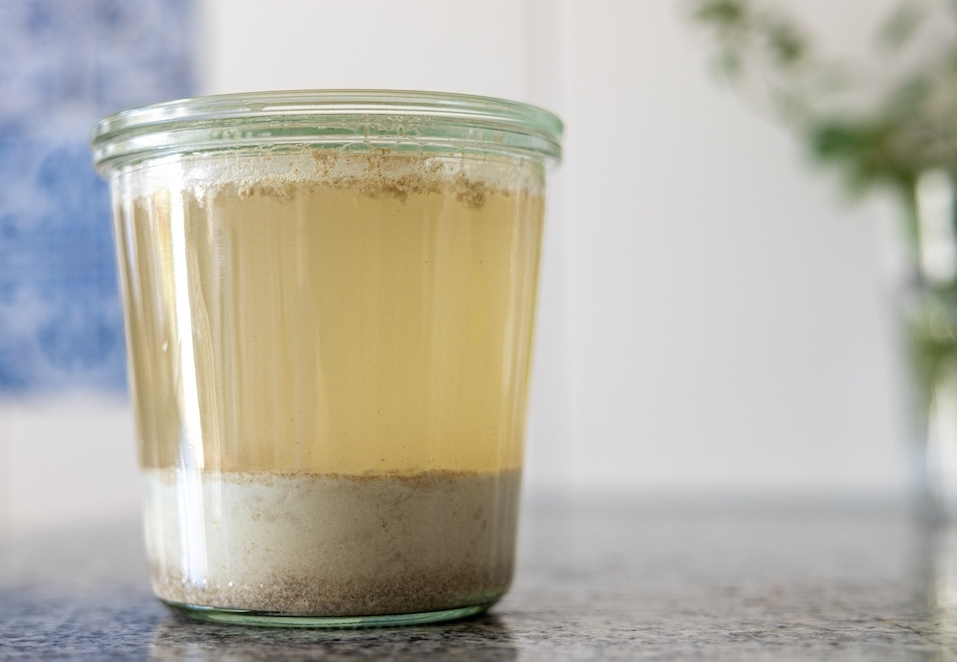
\includegraphics[width=0.5\textwidth]{sourdough-starter-liquid.jpg}
  \caption[Levain liquide]{Un levain liquide a un haut niveau de
      l'eau. La grande quantité d'eau stimule les bactéries productrices d'acide lactique.
      Au bout d'un moment, le liquide et la farine commencent à se séparer. Les bulles sur le
      côté de la farine indiquent que le levain est prêt à être utilisé.}%
  \label{fig:liquid-sourdough-starter}
\end{center}
\end{figure}


\begin{figure}[!htb]
\begin{center}
  \begin{tikzpicture}[node distance = 5cm, auto]
  \node [start] (init) {Take your regular or stiff starter};
  \node [block, right of=init] (feed_new_ratio) {Mix \qty{1}{\gram} existing starter, \qty{5}{\gram} flour and \qty{25}{\gram} water};
  \node [decision, below of=feed_new_ratio, node distance=5cm] (ready_signs) {Sour yogurty smell and bubbles visible on flour?};
  \node [block, right of=ready_signs, node distance=4cm] (feed_again) {Feed again using 1:5:25 ratio};
  \node [block, left of=ready_signs, node distance=5cm] (last_feed) {Feed one last time};
  \node [success, below of=last_feed, node distance=4cm] (bread_dough) {Make bread dough};
  \path [line] (init) -- (feed_new_ratio);
  \path [line] (feed_new_ratio) -- node{Wait \qty{24}{\hour}} (ready_signs);
  \path [line] (feed_again) -- node[anchor=east]  {} ++(2.2,0) |- (feed_new_ratio);
  \path [line] (ready_signs) -- node{no} (feed_again);
  \path [line] (ready_signs) -- node[above=2pt]{~yes} (last_feed);
  \path [line] (last_feed) -- node{after \qtyrange{6}{12}{\hour}} (bread_dough);
  \draw [thick, ->] ($ (feed_again.north) +(0.7cm, 1cm)$) arc (-45:220:1cm);
  \node [anchor=north, text width=5em] at ($(feed_again.north west)+(1.8cm, 2.3cm)$) {Repeat 3~times};
  
\end{tikzpicture}

  \caption[Conversion en un levain liquide]{Le processus pour convertir votre régulier
      ou levain rigide en un levain liquide. L'ensemble du processus prend environ 3
      jours. Plus vous maintenez votre levain au niveau d'hydratation suggéré,
      plus vos micro-organismes s'adaptent. Il est recommandé de
      garder une sauvegarde de votre levain original car l'environnement liquide sélectionnera des micro-organismes anaérobies. Cela stimule les bactéries qui créent de l'acide lactique plutôt que de l'acide acétique. L'acidité résultante sera perçue comme
      plus douce.}%
  \label{fig:liquid-starter-conversion}
\end{center}
\end{figure}

Le levain liquide est fait à une hydratation d'environ \qty{500}{\percent}. Cela signifie
que le levain a beaucoup plus d'eau que de farine. La couche supplémentaire d'eau sur
le dessus de la farine change le microbiome de votre levain.En introduisant cette couche d'eau, moins d'oxygène est disponible tout au long du processus de fermentation. Cela signifie que votre levain ne produira plus d'acide acétique. Les bactéries lactiques hétérofermentaires vont prospérer dans cet environnement. Voilà une petite astuce pour changer le profil de saveur de votre levain de vinaigré à lactique. Votre levain va développer des notes crémeuses laitières. De façon intéressante, lorsque l'hydratation change de nouveau, votre levain va conserver le profil de saveur du levain liquide, mais bénéficiera à nouveau d'une activité de levure accrue. La conversion du levain liquide est irréversible. Il est donc conseillé de conserver une copie de sauvegarde de votre levain ferme ou régulier.

Pour commencer la conversion, prenez environ 1 gramme de votre levain, mélangez avec 5 grammes de farine et 25 grammes d'eau. Remuez bien le tout. Après quelques minutes, la farine va commencer à se déposer au fond de votre pot. Répétez ce processus pendant quelques jours. Secouez doucement le levain pour voir si vous pouvez voir de petites bulles de CO2 se déplacer dans le liquide. C'est un bon signe que votre levain est prêt. Utilisez votre nez pour sentir le levain. Il devrait avoir une note de saveur crémeuse laitière.

Comme vous avez plus d'activité bactérienne, ce levain fonctionne mieux avec une farine très forte qui peut résister à une longue période de fermentation. Utiliser ce levain avec une farine de blé faible ne fonctionnera pas. Si vous ne vous souciez pas de cuire un pain à la structure libre, alors vous pouvez facilement utiliser ce levain avec un moule à pain. Ce levain fonctionne également très bien pour faire une pâte à crêpes robuste. Pour l'utiliser, je secoue le contenant du levain jusqu'à ce que je voie que tous les ingrédients sont homogénéisés. Ensuite, j'utilise environ 5% de celui-ci en termes de calcul du boulanger. Donc pour 1000 grammes de farine, c'est environ 50 grammes de levain liquide. Comme il est très liquide, vous devez inclure les 50 grammes dans votre calcul de liquide. Je traite généralement le levain directement comme un liquide dans les recettes. Donc si la recette demande 600 grammes d'eau et que j'utilise 50 grammes de levain, alors je procède et n'utilise que 550 grammes d'eau.

Ce type de levain est également un excellent combattant contre la moisissure. Comme vous supprimez l'oxygène de l'équation, la moisissure aérobie ne peut pas bien se développer. Si votre levain a un problème de moisissure, alors la conversion en liquide pourrait être le remède. Prenez une partie de votre levain où vous soupçonnez la présence de moisissure. Appliquez la conversion comme mentionné précédemment. La moisissure va probablement sporuler car elle manque de nourriture. Avec chaque nouveau repas, vous réduisez les spores de moisissure. Les spores ne peuvent plus se réactiver car elles ne peuvent pas le faire dans les conditions anaérobies.

Le liquide sur le dessus de votre levain est une excellente ressource que vous pourriez utiliser pour faire des sauces. Si vous avez l'impression que vous aimeriez ajouter un peu d'acidité, égouttez la partie liquide sur votre levain et utilisez-la. Je l'ai utilisé de nombreuses fois pour faire des sauces piquantes lacto-fermentées.

\section{Levain ferme}
\label{section:levain-ferme}

\begin{figure}[!htb]
  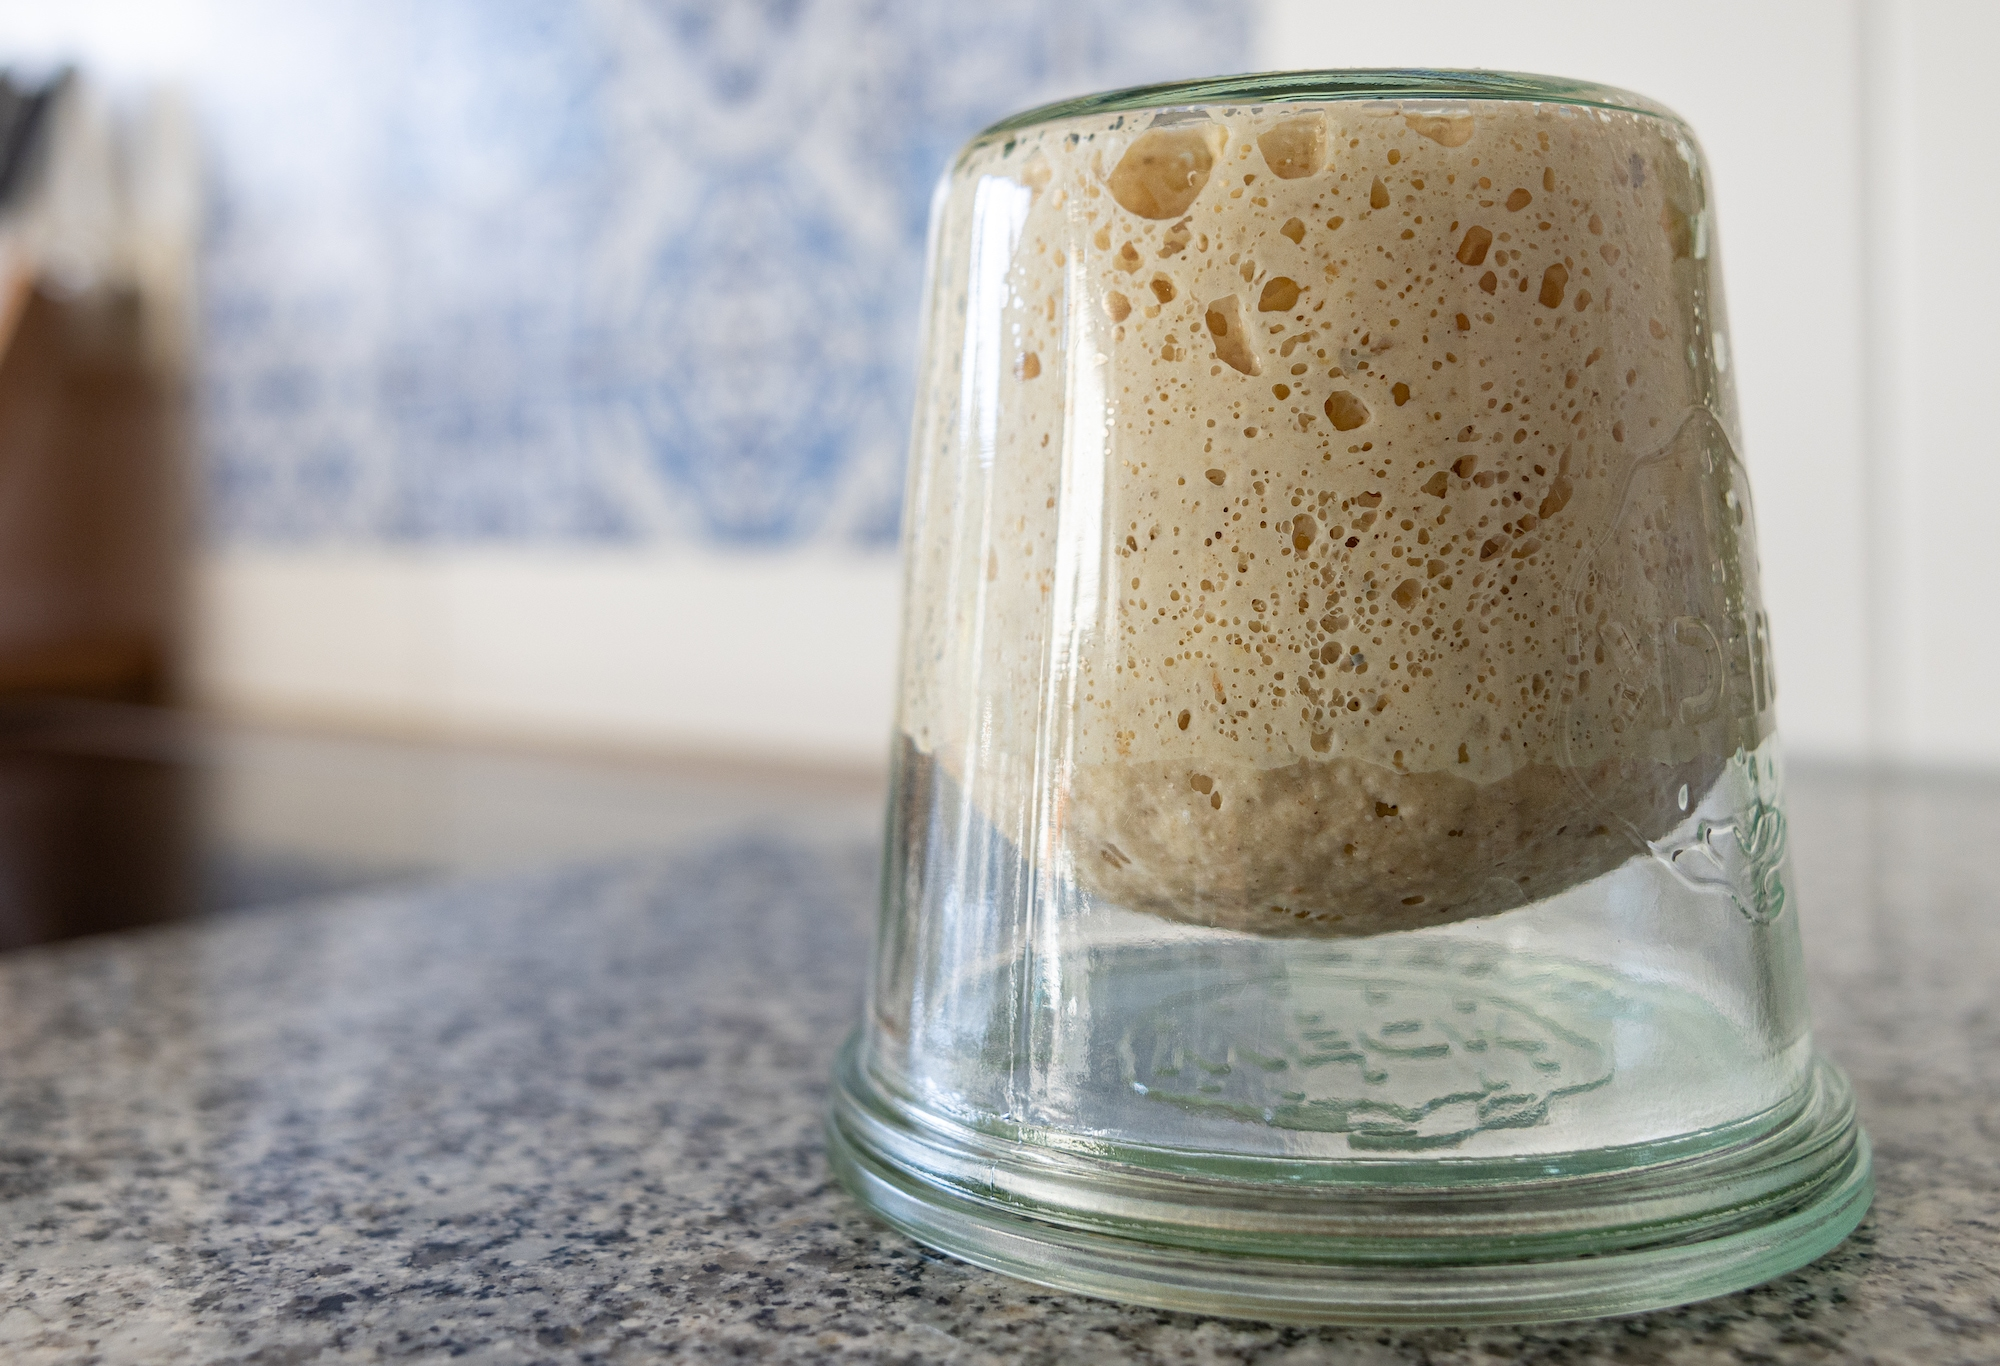
\includegraphics[width=\textwidth]{sourdough-starter-stiff.jpg}
  \caption[Levain ferme à l'envers]{Un levain ferme que j'ai utilisé pour faire une pâte à Stollen pour Noël. Notez les bulles sur le bord du récipient. La pâte ne tombe pas du pot.}
  \label{fig:levain-ferme-sourdough-starter}
\end{figure}Le levain dur est le plus sec de tous les levains. Il a une hydratation
d'environ \qtyrange{50}{60}{\percent}. Donc pour \qty{100}{\gram} de farine vous utilisez environ
\qtyrange{50}{60}{\gram} d'eau. Si vous ne pouvez pas mélanger la farine et l'eau parce que le
mélange est trop sec, vous devez augmenter la quantité d'eau. C'est souvent
le cas lorsque vous utilisez de la farine de blé entier/seigle pour préparer votre levain. Plus
votre farine contient de son, plus votre farine peut absorber d'eau. Le levain dur
devrait avoir une consistance comparable à celle de la pâte à pâtes ou à pizza. Lorsque
vous mélanger le levain il ne doit y avoir aucun grumeau de farine. Testez en plaçant
le levain sur votre plan de travail de cuisine. Lorsque vous le soulevez, il devrait légèrement coller
à la surface de votre comptoir. Ce test indique que vous avez suffisamment hydraté la farine.
Lorsque le mélange est trop sec, la vitesse de fermentation est grandement réduite et
le levain semblera inactif. Le levain devrait être beaucoup plus sec
qu'un levain ordinaire, mais aussi pas trop sec. Reportez-vous à la figure~\ref{fig:stiff-starter-dry-check}
pour un exemple visuel du niveau d'hydratation requis du levain. 

\begin{figure}[!htb]
  \includegraphics[width=\textwidth]{stiff-starter-dry-check.jpg}
  \caption[Un levain trop sec et parfaitement hydraté]{Une image vous montrant un
      levain dur qui est trop sec et un qui est parfaitement hydraté. Le
      levain ne doit pas contenir de grumeaux de farine et coller légèrement à votre
      plan de travail. Le levain sur la photo est fait avec de la farine de blé entier.}%
  \label{fig:stiff-starter-dry-check}
\end{figure}

\begin{figure}[!htb]
\begin{center}
  \begin{tikzpicture}[node distance = 4cm, auto]
  \node [start] (init) {Take your regular or liquid starter};
  \node [block, right of=init, node distance = 4cm] (feed_new_ratio) {Mix \qty{10}{\gram} existing starter, \qty{50}{\gram} flour and \qty{25}{\gram} water};
  \node [decision, right of=feed_new_ratio, node distance=5cm] (too_dry) {Starter very dry, hard to mix?};
  \node [block, right of=too_dry, node distance=4cm] (add_water) {Add more water};
  \node [block, below of=too_dry] (next_day) {Wait\\ \qty{24}{\hour}};
  \node [block] at (feed_new_ratio |- next_day) (feed_again) {Feed again using 1:5:2.5 ratio};
  \node [decision, below of=next_day, node distance=3.5cm] (ready_signs) {Size increase and sour smell?};
  \node [block] at (ready_signs -| add_water) (last_feed) {Feed one last time};
  \node [success, below of=last_feed, node distance=3cm] (bread_dough) {Make bread dough};
  \path [line] (init) -- (feed_new_ratio);
  \path [line] (feed_again) -- (feed_new_ratio);
  \path [line] (next_day) -- (ready_signs);
  \path [line] (ready_signs) -- node{no} (feed_again |- last_feed) |- (feed_again.south);
  \path [line] (ready_signs) -- node{yes} (last_feed);
  \path [line] (last_feed) -- node{after \qtyrange{6}{12}{\hour}} (bread_dough);
  \path [line] (feed_new_ratio) -- (too_dry);
  \path [line] (add_water.north) -- node{} ++(0, 1.3) -| (too_dry.north);
  \path [line] (too_dry) -- node{no} (next_day);
  \path [line] (too_dry) -- node{yes} (add_water);
  \path [line] (ready_signs) -- node{yes} (last_feed);
  \draw [thick, <-] ($ (feed_again.east) +(2.1cm, 0.7cm)$) arc (-45:220:1cm);
  \node [anchor=north, text width=5em] at ($(feed_again.east)+(2cm, 2cm)$) {Repeat 3~times};
\end{tikzpicture}

  \caption[Conversion en levain dur]{Le processus pour convertir votre levain
      ordinaire en levain dur. L'ensemble du processus prend environ 3 jours. Le
      plus vous maintenez votre levain au niveau d'hydratation suggéré, le
      plus vos microorganismes s'adaptent. Le levain dur stimule l'
      activité des levures de votre levain. Le guide utilise un
      niveau d'hydratation de \qty{50}{\percent} pour le levain. Si la pâte est trop
      raide, envisagez d'augmenter cela à \qty{60}{\percent}.}%
  \label{fig:stiff-starter-conversion}
\end{center}
\end{figure}

Dans un environnement plus rigide, la levure prospère davantage. Cela signifie que vous aurez
plus de production de \ch{CO2} et moins de production d'acide. Dans mes tests, c'est un élément déterminant,
surtout si vous utilisez des farines au gluten plus faible. Les farines de blé dans
mon pays d'origine, l'Allemagne, ont tendance à être plus pauvres en gluten. Pour que le blé forme du gluten, des conditions chaudes
sont préférées~\cite{gluten+development+temperatures}. Lorsque je suivais des recettes
d'autres boulangers, je ne parvenais jamais à obtenir des résultats similaires. Lorsque je suivais
les temps indiqués, mes pâtes s'effondraient simplement et devenaient super collantes. Ce n'est que lorsque j'ai commencé à acheter de la farine de blé plus
coûteuse que mes résultats ont commencé à changer. Comme tout le monde ne peut pas se permettre
ces farines spéciales pour la boulangerie et en raison de leur disponibilité limitée, je suis tombé sur le
levain dur. J'ai fait plusieurs tests où j'ai utilisé la même quantité de
levain et de farine. Je n'ai changé que l'hydratation entre tous les levains.
Je procéderais ensuite à placer un ballon sur le dessus de chacun des bocaux. Le bocal de
levain dur était clairement le plus gonflé. Le levain ordinaire
arrivait en deuxième position. Le levain liquide finissait en troisième position avec beaucoup moins de production de \ch{CO2}.

\begin{figure}[!htb]
  \includegraphics[width=\textwidth]{stollen}
  \caption[\emph{Stollen} de Noël]{Un \emph{Stollen} de Noël allemand fait
      avec un levain dur au lieu de levure.}%
  \label{fig:stollen}
\end{figure}J'ai ensuite procédé et acheté une farine à gâteau bon marché dans mon supermarché à proximité.
Cette farine m'avait précédemment causé de gros maux de tête. J'ai fait un pain au levain
exactement comme je le fais normalement. J'ai dû réduire un peu l'hydratation car une faible
farine de gluten n'absorbe pas autant d'eau. Puis j'ai remplacé le levain par
le levain dur. La pâte se sentait incroyable et était soudainement capable de résister à
une période de fermentation beaucoup plus longue. Le pain avait une grande poussée au four et avait un goût
très doux. Je cherche encore à trouver une explication précise de pourquoi la partie levure de
la pâte est plus active. Peut-être qu'elle ne l'est pas. Il se pourrait aussi que les bactéries
soient inhibées par le manque d'eau.

Lors de la confection du levain dur, commencez par utiliser environ \qty{50}{\percent}
d'eau. Si vous utilisez une farine complète, ou une farine forte, envisagez d'aller
jusqu'à \qty{60}{\percent}. Tous les ingrédients doivent se mélanger très bien. Il
ne devrait pas rester de farine émiettée. C'est une erreur courante que j'ai vue quand
les gens essayaient de faire le levain dur. Oui, il doit être sec, mais pas à un
point où c'est un bloc de ciment. Si vous avez déjà fait une pâte à pâtes, cette
pâte devrait avoir exactement la même consistance.

Pour évaluer si votre levain dur est prêt, recherchez une calotte. Cherchez aussi
des poches d'air sur les côtés de votre récipient. Utilisez votre nez pour sentir le
levain. Il devrait avoir une odeur douce. Il a aussi tendance à sentir beaucoup plus
alcool que les autres levures.

Lors de l'utilisation d'un levain dur, utilisez environ \qtyrange{1}{20}{\percent} en fonction de
la maturité de votre levain. En été, j'utilise généralement environ
\qty{10}{\percent} et en hiver environ \qty{20}{\percent}. De cette façon, vous pouvez
contrôler également la vitesse de fermentation.
Mélanger le levain peut être un peu ennuyeux car il se mélange difficilement avec
le reste de la pâte. Dans ce cas, vous pouvez essayer de dissoudre le levain dans l'eau
que vous allez utiliser pour votre pâte. Cela facilitera beaucoup le mélange.


\section{Lievito madre ou pasta madre}

Le lievito madre, également connu sous le nom de pasta madre, appartient à la même catégorie que
le levain dur. Après des heures de recherche, je n'ai pas
trouvé de différence entre la pasta madre et le lievito madre. Les deux termes semblent être
utilisés de manière interchangeable dans la littérature.

Dans de nombreuses recettes, ce levain est fait directement
à partir de fruits secs ou frais. Vous pouvez également faire un levain à partir de feuilles de votre
jardin. Comme décrit précédemment, la levure sauvage et les bactéries consomment le glucose
des feuilles des plantes. Toutes les options fonctionnent. Lors de la confection d'un levain directement
à partir de fruits secs, il vous manque parfois la partie bactérienne de la fermentation.
L'acidité est très importante pour nettoyer votre levain des éventuels
pathogènes. Si vous décidez de faire votre levain à partir de fruits, assurez-vous qu'il
s'acidifie correctement lors de la confection d'une pâte. Un outil comme un pH-mètre peut être d'une grande
aide. Généralement, plus le pH est bas, plus l'acidité est élevée. L'acidité
doit être inférieure à 4.2 pour savoir que votre levain produit suffisamment d'acidité.

Certains boulangers nettoient le lievito madre dans un bain d'eau. C'est censé
éliminer l'excès d'acidité. Dans mes propres expériences, je n'ai pas été capable de confirmer
cette méthodologie. L'acidité reste la même. La seule raison pour laquelle cela pourrait
avoir du sens est si vous essayiez également de stimuler les micro-organismes anaérobies. Cependant, alors le
levain devrait rester dans cet environnement pendant un certain temps et pas seulement
quelques heures.
La cuisson avec du levain est simple. Ce n'est que de la farine et de l'eau. Lorsque vous voyez une recette
d'un boulanger expérimenté, vous vous demandez, Attend, c'est tout? Il n'y a rien de plus
à cela? J'ai l'impression que c'est peut-être la raison pour laquelle certains boulangers ont des procédures d'alimentation si compliquées. Ils se réfugient dans plusieurs nourritures par jour à un certain ratio donné.
Cela rend le boulanger un peu plus élitiste. Bien sûr, avec le temps, comme
de plus en plus de gens suivent cette procédure, elle devient une prophétie auto-réalisatrice.
Plus vous devenez expérimenté, plus les chances sont grandes qu'un guide d'alimentation de départ bidon
vous récompense avec de beaux résultats. La raison, cependant, n'est
pas dans la routine de départ. La raison est que vous comprenez mieux la fermentation
et devenez meilleur à lire les signes de votre pâte.

Si je devais choisir un type de levain, je choisirais le levain dur. Dans de nombreux cas,
il vous fournira des résultats constamment excellents avec peu d'effort.
D'après mon expérience, vous pouvez réaliser n'importe quelle pâte à base de levure et simplement remplacer
la levure directement par le levain dur. Vous serez capable
d'obtenir des résultats encore meilleurs avec le levain dur.

Enfin, peu importe le type de levain que vous choisissez, vous pouvez contrôler à quel point
vous voulez que votre pâte soit aigre. Plus vous prolongez la fermentation, plus
l'acidité va s'accumuler. La seule différence est que pour une augmentation donnée
de volume, le levain dur produira le moins d'acidité. Donc pour une
augmentation de volume de 100\%, le levain liquide a produit le plus d'acidité,
suivi du levain régulier puis du levain dur. Si vous attendez assez
longtemps, le levain dur aura produit la même quantité d'acidité que les
autres levains. Mais avant de le faire, il aura également produit beaucoup plus de \ch{CO2}. Si
vous aimez la saveur aigre, vous devez prolonger votre fermentation. Cela signifie également
que vous devez soit cuire dans un moule à pain, soit avoir une farine de gluten très forte
qui est capable de résister à de longs temps de fermentation.